\documentclass[a4paper,10pt]{article}

\usepackage[latin1]{inputenc}
\usepackage[spanish]{babel}
\usepackage{fontenc}
\usepackage{graphicx}
\usepackage{url}
\usepackage{verbatim}
\author{Santiago Videla}
\title{Especificaci\'on de Dise\~no de Software}
\pagestyle{headings}
\date{12 de octubre de 2010}
\begin{document}
\maketitle
\newpage
\tableofcontents
\newpage
\section{Introducci\'on}
  \subsection{Prop\'osito}

El prop\'osito de este documento es la especificaci\'on de
dise\~no de software para la primer versi\'on del producto ``vac-o''.

La confecci\'on de este documento se enmarca dentro del desarrollo de la tesis
de grado de la carrera Lic. en Cs. de la Computaci\'on de la FaMAF - UNC,
\textbf{``Dise\~no de vacunas atenuadas con menor probabilidad de sufrir
reversi\'on a la virulencia''} a cargo de Santiago Videla, con la direcci\'on
de la Dra. Laura Alonso i Alemany (FaMAF) y la colaboraci\'on de Daniel
Gutson (FuDePAN).

El documento esta dirigido a las personas involucradas en el desarrollo de la
tesis como as\'i tambi\'en a los colaboradores de FuDePAN que eventualmente
podr\'ian participar en las etapas de desarrollo y mantenimiento del software.

\subsection{Descripci\'on general del documento}

En la secci\'on~\ref{considerations} se mencionan los objetivos, la
metodolog\'ia adoptada y las dependencias del dise\~no.

En la secci\'on~\ref{architecture} se muestra la arquitectura del
sistema con sus principales componentes e interacciones.

En la secci\'on~\ref{hld} se presenta el dise\~no de alto nivel del sistema,
sus interfaces y paquetes principales.

En la secci\'on~\ref{lld} se presenta el dise\~no de bajo nivel del sistema,
las clases concretas y sus relaciones para cada paquete.

\section{Consideraciones de Dise\~no}
\label{considerations}

\subsection{Objetivos}

Principalmente se pretende lograr un dise\~no que cumpla con los principios
fundamentales del dise\~no orientado a objetos, com\'unmente conocidos por el
acr\'onimo ``SOLID'' \cite{martin00}.

En particular, se pone especial \'enfasis en respetar los principios OCP
(\textit{Open-Closed Principle}) y DIP (\textit{Dependency Inversion Principle})
debido a su importancia para obtener un sistema que sea f\'acilmente extensible
y configurable con el fin de satisfacer las necesidades de los usuarios.
  
\subsection{Metodolog\'ia}

La metodolog\'ia utilizada para realizar el an\'alisis y descripci\'on del
dise\~no se denomina ``Dise\~no dirigido por responsabilidades''
\cite{wirfsbrok03}. Esta t\'ecnica se enfoca en \textit{qu\'e} acciones
(responsabilidades) deben ser cubiertas por el sistema y que objetos ser\'an los
responsables de llevarlas a cabo. \textit{C\'omo} se realizara cada acci\'on,
queda en un segunda plano.

\subsection{Dependencias}

Se asume para la confecci\'on de este dise\~no, el acceso a diferentes
librer\'ias externas que ser\'an fundamentales para el correcto funcionamiento
del sistema en su conjunto. Respetando la metodolog\'ia adoptada, no se har\'a
referencia directa a una u otra librer\'ia, sino a los servicios que las mismas
debe ser capaces de proveer al sistema.

\subsection{Herramientas y convenciones}

Se utiliza UML\cite{uml} como lenguaje de modelado y ArgoUML\cite{argoUML}
como herramienta para la confecci\'on de diagramas. Adem\'as se adopta la
convenci\'on de nombrar a las interfaces anteponiendo una \textit{``I''} al
nombre de la clase concreta que la implementa (interface: \textit{``IPersona''},
clase concreta: \textit{``Persona''}).

\section{Arquitectura del Sistema}
\label{architecture}

En la Figura~\ref{uml:architecture} se presenta un diagrama de la
arquitectura del sistema y la interacci\'on entre sus componentes principales.
A continuaci\'on se da una breve descripci\'on de cada uno de ellos:

  \begin{itemize}
   \item \textbf{Main:} Representa el componente principal en t\'erminos de
ejecuci\'on del sistema. Comprende principalmente, la inicializaci\'on y
configuraci\'on de otros componentes.

   \item \textbf{Plugin:} Representa la implementaci\'on de las
caracter\'isticas propias de la vacuna que se desea optimizar. Brinda
informaci\'on de configuraci\'on inicial como as\'i tambi\'en, los criterios
para evaluar una secuencia.

   \item \textbf{CombinatoryEngine:} Representa el motor combinatorio del
sistema encargado de encontrar, nuevas secuencias que sean candidatas a
optimizar la atenuaci\'on de la vacuna.

   \item \textbf{QAEngine:} Representa el motor de control de calidad del
sistema encargado de decidir, si una secuencia candidata pasa o no dicho
control.

   \item \textbf{Ranker:} Representa el componente encargado de mantener un
``ranking'' de secuencias.

   \item \textbf{libRNA:} Representa el componente que provee al sistema
funcionalidades para la manipulaci\'on de secuencias de ARN (``folding'' directo
e inverso) utilizando librer\'ias externas (Vienna Package, UNAFold, entre
otras)

  \end{itemize}

  \begin{figure}
  \centering
  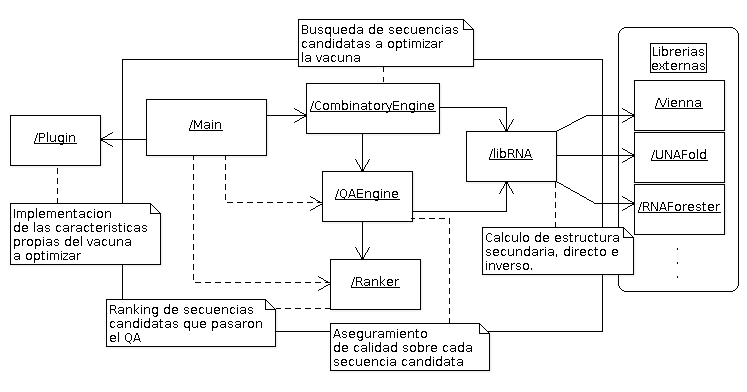
\includegraphics[scale=0.5]{architecture.png}  
  \caption{UML - Arquitectura}
  \label{uml:architecture}
  \end{figure}

\section{Dise\~no de alto nivel}
\subsection{Interfaces - Responsabilidades - Colaboradores}
\begin{figure}
  \centering
  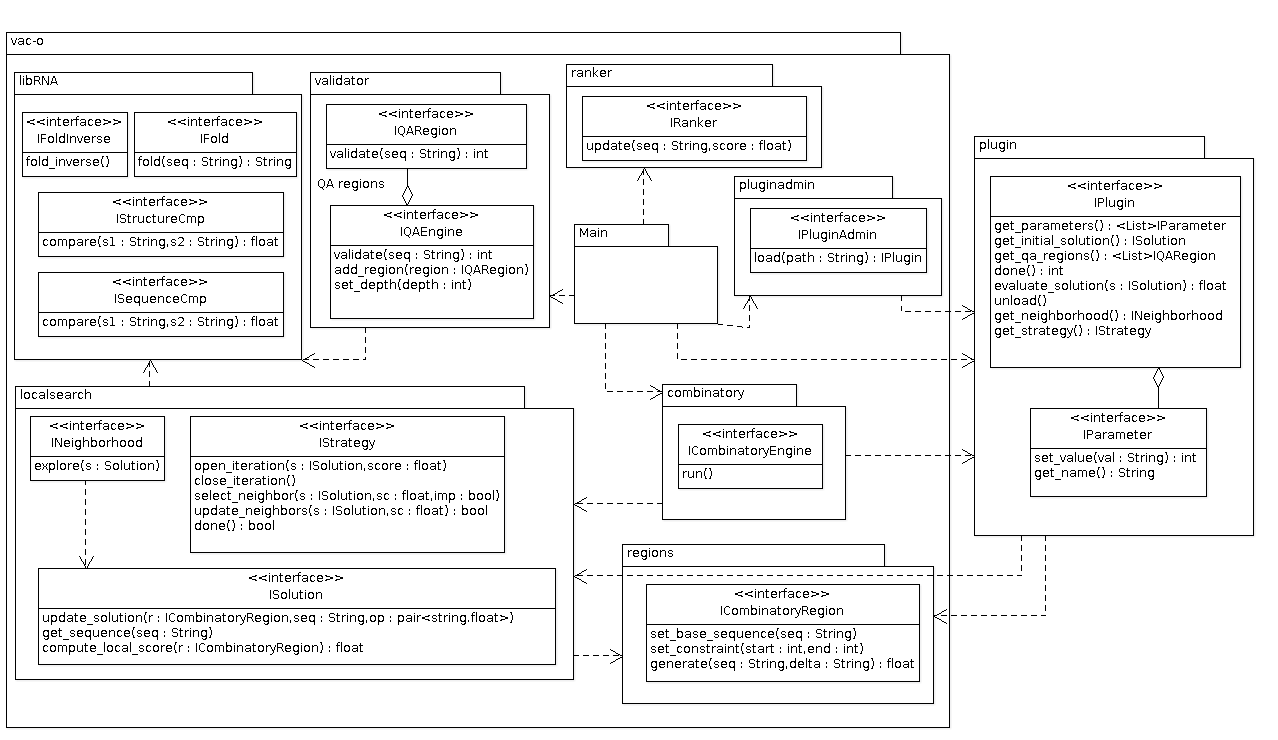
\includegraphics[scale=0.5, angle=90]{hld.png}  
  \caption{UML - Interfaces}
  \label{uml:1}
\end{figure}

  \subsubsection{IPluginAdmin}
    \paragraph{Responsabilidad:} Administrar las extensiones del sistema
(archivos \textit{.so}).    
      \begin{enumerate}
       \item Cargar extensi\'on.       
      \end{enumerate}    

  \subsubsection{IPlugin}
    \paragraph{Responsabilidad:} Brindar la informaci\'on y servicios
particulares para una vacuna determinada.    
      \begin{enumerate}
       \item Proveer la lista de par\'ametros requeridos por la extensi\'on.
       \item Proveer la secuencia de ARN que se encuentra en la cepa vacunal.
       \item Proveer las regiones combinatorias que se deben usar para buscar
mejoras a la vacuna.
       \item Proveer el umbral que se debe usar para determinar la bondad de las
secuencias obtenidas de las regi\'ones combinatorias.
       \item Proveer las regiones de validaci\'on que se deben usar para
realizar el control de calidad.
       \item Determinar si se continua buscando secuencias o no.
       \item Evaluar las secuencias candidatas.
       \item Descargar la extensi\'on.
      \end{enumerate}
    \paragraph{Colaboradores:}
      \begin{enumerate}
       \item \textbf{BioPP:} Calculo de distancias entre secuencias.
       \item \textbf{LibPlugin}: Factories de regiones combinatorias y de
validaci\'on.
      \end{enumerate}

  \subsubsection{ICombinatoryRegion}
    \paragraph{Responsabilidad:} Calcular las secuencias que mantengan
determinadas propiedades de una secuencia original.    
      \begin{enumerate}
       \item Devolver la siguiente secuencia.
       \item Evaluar la bondad de una secuencia.
      \end{enumerate}
    \paragraph{Colaboradores:}
      \begin{enumerate}
       \item \textbf{BioPP:} Calculo de secuencias que mantengan una propiedad
determinada (estructura secundaria, c\'odigo gen\'etico, etc).
      \end{enumerate}

  \subsubsection{ICombinatoryEngine}
    \paragraph{Responsabilidad:} Generar secuencias candidatas a partir de las
variantes generadas de cada regi\'on combinatoria.       
      \begin{enumerate}       
       \item Inicializar las regiones combinatorias.
       \item Devolver la siguiente secuencia candidata.
      \end{enumerate}
    \paragraph{Colaboradores:}
      \begin{enumerate}
       \item \textbf{ICombinatoryRegion:} Consulta la siguiente secuencia de
cada regi\'on combinatoria.
      \end{enumerate}

  \subsubsection{IQAMutator}
    \paragraph{Responsabilidad:} Generar mutaciones de una secuencia
utilizando alg\'un criterio (todas las mutaciones posibles, $N$
mutaciones aleatorias, etc).
      \begin{enumerate}
       \item Devolver la siguiente mutaci\'on.
      \end{enumerate}    

  \subsubsection{IQAValidator}
    \paragraph{Responsabilidad:} Decidir si una secuencia satisface o
mantiene determinadas propiedades.
    \paragraph{Colaboradores:}
      \begin{enumerate}
       \item \textbf{BioPP:} Calculo y comparaci\'on de estructura secundaria o
conteo de nucle\'otidos
      \end{enumerate}

  \subsubsection{IQARegion}
    \paragraph{Responsabilidad:} Realizar el control de calidad para una
regi\'on de validaci\'on.
      \begin{enumerate}
       \item Calcular y validar mutaciones acumuladas de la regi\'on hasta
alcanzar la profundidad deseada.
      \end{enumerate}
    \paragraph{Colaboradores:}
      \begin{enumerate}
       \item \textbf{IQAMutator:} Consulta la siguiente mutaci\'on.
       \item \textbf{IQAValidator:} Consulta si una mutaci\'on determinada es
valida o no.
      \end{enumerate}

  \subsubsection{IQAEngine}
    \paragraph{Responsabilidad:} Realizar el control de calidad para una
secuencia candidata.
      \begin{enumerate}       
       \item Inicializar regiones de validaci\'on.
       \item Determinar si una secuencia candidata aprueba o no el control de
calidad para todas sus regiones de validaci\'on.
      \end{enumerate}
    \paragraph{Colaboradores:}
      \begin{enumerate}
       \item \textbf{IQARegion:} Consulta si la regi\'on de validaci\'on aprueba
o no el control de calidad.
      \end{enumerate}

  \subsubsection{IRanker}
    \paragraph{Responsabilidad:} Mantener un \textit{ranking} de secuencias en
base al puntaje asignado a cada una.       
    \paragraph{Colaboradores:}
      \begin{enumerate}
       \item \textbf{IPlugin:} Consulta el puntaje para una secuencia
determinada.
      \end{enumerate}

\begin{comment}
  \subsection{Interface}
    \paragraph{Responsabilidad:}    
      \begin{enumerate}
       \item 
      \end{enumerate}
    \paragraph{Colaboradores:}
      \begin{enumerate}
       \item 
      \end{enumerate}
\end{comment}

\section{Dise\~no de bajo nivel}
\label{lld}  
    \begin{figure}
      \centering
      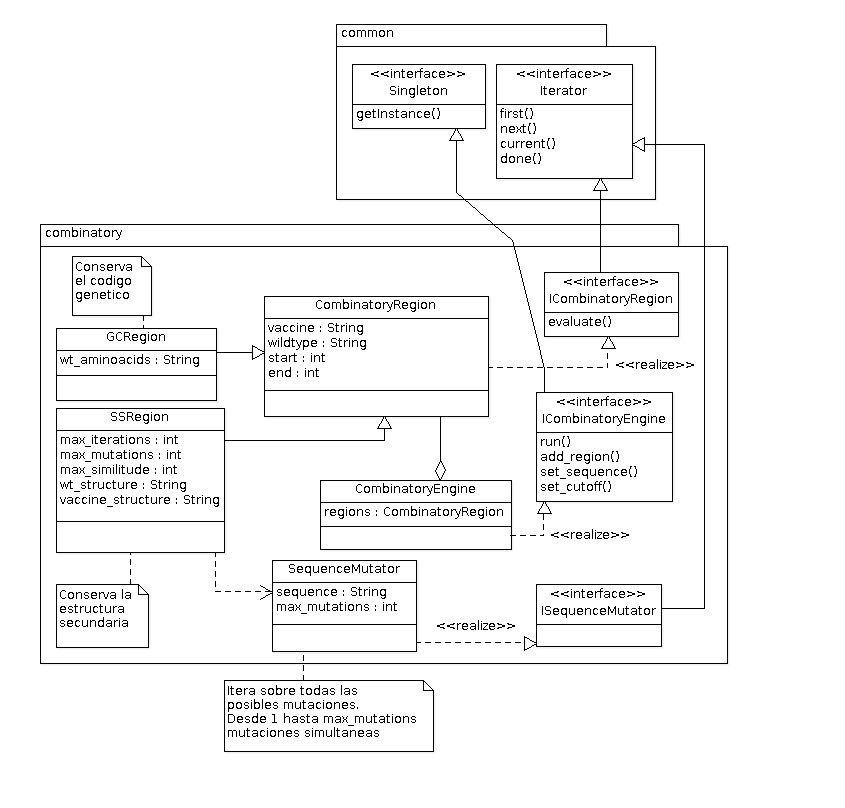
\includegraphics[scale=0.5]{lld-combinatory.png}  
      \caption{UML - Combinatory}
      \label{uml:2}
    \end{figure}

    \begin{figure}
      \centering
      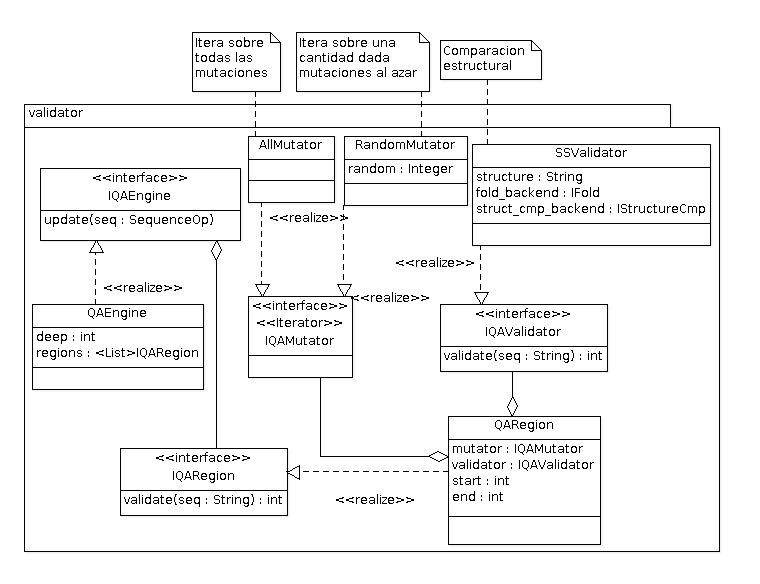
\includegraphics[scale=0.5]{lld-validator.png}  
      \caption{UML - Validator}
      \label{uml:3}
    \end{figure}

\begin{thebibliography}{9}  
  \bibitem{martin00}
  Design Principles and Design Patterns. Robert C. Martin, 2000.\\
  \url{www.objectmentor.com}
  
  \bibitem{wirfsbrok03}
  Rebecca Wirfs-Brock and Alan McKean. Object Design: Roles, Responsibilities
and Collaborations, Addison-Wesley, 2003

  \bibitem{uml}
  Unified Modeling Language: \url{http://www.uml.org/}

  \bibitem{argoUML}
  ArgoUML: \url{http://argouml.tigris.org/}

  
\end{thebibliography}
\end{document}
